\chapter{The Reference Sun as a Lighting Fixture}
\label{chap:sun}

This chapter turns the Sun into a set of numbers a lighting specialist can compare a lamp against: how much light it delivers, in lux; how sharp the shadows it casts are, in millimetres of penumbra per metre; and why those two together force a collimated beam rather than simply a bright one.

\section{Nominal solar constants}

Three constants are taken from IAU 2015 Resolution B3, which fixes nominal values for solar quantities so that published work does not drift as measurements are refined \cite{prsa2016iau}:

\begin{table}[!ht]
\centering
\small
\caption[Nominal solar constants used in this document]{Nominal solar constants, IAU 2015 Resolution B3 \cite{prsa2016iau}. The total solar irradiance is quoted there as a solar-cycle-23 mean of $1361 \pm 0.5$~W/m\textsuperscript{2}.}
\label{tab:solar-constants}
\begin{tabularx}{\textwidth}{p{0.235\textwidth} p{0.095\textwidth} p{0.185\textwidth} X}
\toprule
\textbf{Quantity} & \textbf{Symbol} & \textbf{Nominal value} & \textbf{Used in this document for} \\
\midrule
Total solar irradiance   & $\mathcal{S}^{\,\mathrm{N}}_{\odot}$ & 1361 W/m\textsuperscript{2}  & Illuminance of the orbital Sun (Sec. \ref{sec:sun-lux}) \\
Solar radius             & $\mathcal{R}^{\,\mathrm{N}}_{\odot}$ & 695\,700 km                 & Angular diameter, shadow sharpness (Sec. \ref{sec:angular}) \\
Solar effective temperature & $\mathcal{T}^{\,\mathrm{N}}_{\mathrm{eff}\odot}$ & 5772 K       & Target colour temperature (Sec. \ref{sec:colour}) \\
Astronomical unit        & $\mathrm{au}$                        & 149\,597\,870.7 km          & Angular diameter (Sec. \ref{sec:angular}) \\
\bottomrule
\end{tabularx}
\end{table}

\section{From watts per square metre to lux}
\label{sec:sun-lux}

\subsection{The conversion}

Applying the definition of luminous flux, Equation \ref{eq:lumen}, to an irradiance distribution rather than a flux gives the illuminance produced by a spectrum $E_{e,\lambda}$:

\begin{equation}
E_v = K_m \int_{0}^{\infty} E_{e,\lambda}(\lambda)\, V(\lambda)\, d\lambda .
\label{eq:lux-from-spectrum}
\end{equation}

Two primary data sets are required to evaluate it, and both are archived in \texttt{Sources/data/}:

\begin{itemize}
    \item $E_{e,\lambda}(\lambda)$, the ASTM E490-00a standard extraterrestrial (AM0) solar spectral irradiance \cite{astm_e490_data}, tabulated from 119.5~nm upward.
    \item $V(\lambda)$, the CIE photopic spectral luminous efficiency function at 1~nm resolution, CIE 018:2019 Table 1 \cite{cie_vlambda}.
\end{itemize}

Numerically integrating the E490 table by the trapezoidal rule gives a total irradiance of $E_e = 1366.1$~W/m\textsuperscript{2}, and integrating the same table weighted by $V(\lambda)$ gives $E_v = 133\,320$~lx. The ratio is the luminous efficacy of extraterrestrial sunlight, Equation \ref{eq:efficacy}:

\begin{equation}
K_{\mathrm{AM0}} = \frac{133\,320~\mathrm{lx}}{1366.1~\mathrm{W/m^2}} = 97.59~\mathrm{lm/W} .
\label{eq:k-am0}
\end{equation}

The E490 table integrates to 1366.1~W/m\textsuperscript{2} rather than the IAU nominal 1361~W/m\textsuperscript{2}, a difference of 0.37\%, because the two were established at different times against different radiometric scales. Since $K$ is a property of the spectral \emph{shape} and is therefore insensitive to that normalisation, the reported illuminance is obtained by applying Equation \ref{eq:k-am0} to the nominal constant:

\begin{equation}
\boxed{\;E_{v,\odot} = K_{\mathrm{AM0}} \cdot \mathcal{S}^{\,\mathrm{N}}_{\odot}
 = 97.59~\mathrm{lm/W} \times 1361~\mathrm{W/m^2} = 132\,800~\mathrm{lx}\;}
\label{eq:sun-lux}
\end{equation}

at normal incidence, outside the atmosphere. This is the single reference figure against which every lamp considered for the dark room is compared.

\subsection{Why the two unit systems differ so much}

Figure \ref{fig:spectrum} shows the mechanism. The Sun radiates across the whole plotted range, but $V(\lambda)$ is non-zero only in a narrow window, so the integrand of Equation \ref{eq:lux-from-spectrum} is confined to the visible band. Table \ref{tab:bands} gives the fraction of AM0 energy in each band of interest.

\begin{figure}[!ht]
\centering
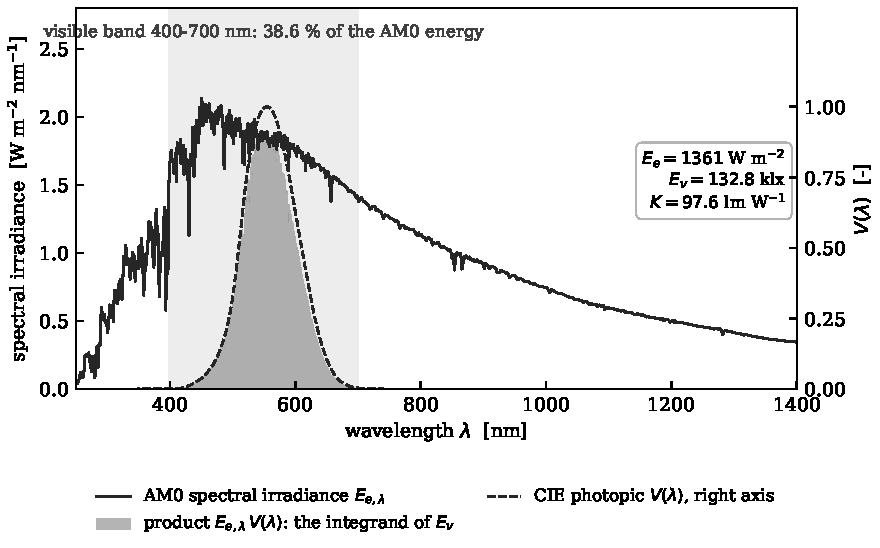
\includegraphics[width=\textwidth]{Images/fig_spectrum_vlambda.pdf}
\caption[AM0 spectral irradiance weighted by the CIE luminous efficiency function]{The AM0 reference spectrum \cite{astm_e490_data}, the CIE photopic luminous efficiency function $V(\lambda)$ \cite{cie_vlambda}, and their product, which is the integrand of Equation \ref{eq:lux-from-spectrum}. The area under the shaded product curve, scaled by $K_m = 683$~lm/W, is the illuminance. Everything the Sun radiates outside the shaded band contributes irradiance but no lux. Generated by \texttt{make\_figures.py} from the archived data files.}
\label{fig:spectrum}
\end{figure}

\begin{table}[!ht]
\centering
\small
\caption[Fraction of AM0 irradiance per wavelength band]{Fraction of the total AM0 irradiance carried by each band, obtained by integrating the E490 table \cite{astm_e490_data}. Computed by \texttt{illumination\_numbers.py}.}
\label{tab:bands}
\begin{tabularx}{\textwidth}{llX}
\toprule
\textbf{Band} & \textbf{Share of $E_e$} & \textbf{Relevance} \\
\midrule
400--700 nm   & 38.6\% & Visible band. Both the Raspberry Pi HQ and Global Shutter cameras carry an infrared filter that reduces sensitivity outside it \cite{raspberrypi_camera_docs}. \\
400--1100 nm  & 66.4\% & Restricted range of the IEC 60904-9 spectral-match classification \cite{iec60904_9_2020}. \\
300--1200 nm  & 77.2\% & Extended range introduced in the 2020 edition, required for class A+ \cite{iec60904_9_2020}. \\
\bottomrule
\end{tabularx}
\end{table}

The practical consequence is that a lamp whose output is heavily weighted toward the infrared can deliver a large irradiance in W/m\textsuperscript{2} while producing few lux and contributing nothing to the image, since the camera's infrared filter discards it. Specifying this experiment in lux rather than W/m\textsuperscript{2} automatically excludes that failure mode.

\section{Colour temperature}
\label{sec:colour}

The Sun's nominal effective temperature is 5772~K \cite{prsa2016iau}, which is why daylight-balanced fixtures are rated near that value. Correlated colour temperature describes the colour of a light source by the temperature of the blackbody radiator it most closely matches; it is not the physical temperature of the lamp. Chapter \ref{chap:sources} shows that every reviewed space laboratory that states a colour temperature uses 5600--6000~K, and Chapter \ref{chap:spec} adopts that range.

\section{Angular diameter and shadow sharpness}
\label{sec:angular}

\subsection{The Sun is not a point source}

From the nominal radius and the astronomical unit, the Sun's angular diameter at 1~au is

\begin{equation}
\alpha_\odot = 2\arctan\!\left(\frac{\mathcal{R}^{\,\mathrm{N}}_{\odot}}{\mathrm{au}}\right)
= 2\arctan\!\left(\frac{695\,700}{149\,597\,870.7}\right) = 0.533^\circ .
\label{eq:angular-diameter}
\end{equation}

This half-degree is what makes orbital shadows look the way they do. A source of finite angular size does not cast a perfectly sharp shadow: behind an occluding edge there is a transition region, the penumbra, which widens with distance from the edge. Figure \ref{fig:penumbra} shows the construction.

\begin{figure}[!ht]
\centering
\begin{tikzpicture}[>=Stealth, font=\small, scale=1.0]

% ---- Extended source ----------------------------------------------------
\draw[line width=2pt] (0,-0.6) -- (0,0.6);
\node[align=center, font=\footnotesize] at (0,-1.35) {extended\\source};
\draw[<->, black!60] (-0.42,-0.6) -- (-0.42,0.6);
\node[font=\footnotesize, rotate=90] at (-0.66,0) {source size};

% ---- Occluder -----------------------------------------------------------
\fill[black!75] (4.0,-2.05) rectangle (4.16,0.0);
\node[align=center, font=\footnotesize] at (4.08,-2.42) {occluding edge};
\fill (4.0,0) circle (1.6pt);

% ---- Rays through the tip ----------------------------------------------
\draw[black!30] (0,0.6) -- (4.0,0);
\draw[black!30] (0,-0.6) -- (4.0,0);
\draw[dashed] (4.0,0) -- (8.0,-0.6);
\draw[dashed] (4.0,0) -- (8.0,0.6);
% unobstructed light passing above the edge
\foreach \y in {0.78,1.02,1.26}{\draw[gray!40,-{Stealth[length=1.5mm]}] (0.25,\y) -- (7.9,\y);}

% angle alpha at the tip
\draw[<->, black!70] (3.0,0.15) arc[start angle=171.5, end angle=188.5, radius=1.01];
\node[font=\footnotesize] at (2.72,0) {$\alpha$};

% ---- Screen -------------------------------------------------------------
\draw[line width=1.1pt] (8.0,-1.7) -- (8.0,1.5);
\node[align=center, font=\footnotesize] at (8.0,1.78) {screen};

% shading of the three regions on the screen
\fill[black!70] (8.02,-1.7) rectangle (8.30,-0.6);
\shade[bottom color=black!70, top color=black!4]
      (8.02,-0.6) rectangle (8.30,0.6);
\fill[black!4, draw=black!25] (8.02,0.6) rectangle (8.30,1.5);

\node[font=\footnotesize, anchor=west] at (8.62,-1.15) {umbra (full shadow)};
\node[font=\footnotesize, anchor=west] at (8.62,0.0)   {penumbra, width $w$};
\node[font=\footnotesize, anchor=west] at (8.62,1.05)  {fully lit};

% brace for w
\draw[decorate, decoration={brace, amplitude=4pt}, black!70]
      (8.40,0.6) -- (8.40,-0.6);

% ---- Distance L ---------------------------------------------------------
\draw[|<->|, black!70] (4.0,-2.75) -- (8.0,-2.75);
\node[font=\footnotesize, fill=white, inner sep=1.5pt] at (6.0,-2.75) {$L$};

\end{tikzpicture}
\caption[Penumbra cast by a source of finite angular size]{Penumbra geometry. The two rays that graze the occluding edge come from opposite edges of the source and therefore diverge by the source's angular size $\alpha$; at a distance $L$ behind the edge they are separated by $w = L\tan\alpha$. The angle $\alpha$ is drawn greatly exaggerated for legibility: at the real solar value of $0.533^\circ$ the two dashed rays would be visually indistinguishable. The construction shown is internally consistent, with $\alpha = 17.1^\circ$ as drawn.}
\label{fig:penumbra}
\end{figure}

\subsection{The penumbra relation}

From the construction in Figure \ref{fig:penumbra}, the penumbra width at a distance $L$ behind the occluding edge is

\begin{equation}
w = L \tan\alpha .
\label{eq:penumbra}
\end{equation}

Evaluating Equation \ref{eq:penumbra} at $\alpha_\odot$ gives $w/L = 9.3$~mm per metre for real sunlight. Table \ref{tab:penumbra} lists the same quantity for the beam divergences that appear later in this document. This relation is the basis of the acceptance test in Chapter \ref{chap:spec}, because it converts an angular specification, which needs optical instruments to verify, into a length measurable with a ruler.

\begin{table}[!ht]
\centering
\small
\caption[Penumbra width per metre for several source angular sizes]{Penumbra width per metre of distance behind the occluding edge, from Equation \ref{eq:penumbra}. Computed by \texttt{illumination\_numbers.py}.}
\label{tab:penumbra}
\begin{tabularx}{\textwidth}{p{0.17\textwidth} X c}
\toprule
\textbf{Angular size $\alpha$} & \textbf{Reference} & \textbf{$w/L$ [mm/m]} \\
\midrule
0.53\textdegree & the real Sun at 1 au, Eq. \ref{eq:angular-diameter} & 9.3 \\
1.00\textdegree & -- & 17.5 \\
1.90\textdegree & collimation angle of the ESA Large Space Simulator beam \cite{esa_lss} & 33.2 \\
2.00\textdegree & limit adopted for LINKU, Chapter \ref{chap:spec} & 34.9 \\
5.00\textdegree & a typical uncollimated spotlight & 87.5 \\
\bottomrule
\end{tabularx}
\end{table}

\section{Why collimation, not merely distance}
\label{sec:falloff}

\subsection{The problem}

The LINKU structure occupies a volume, not a plane. A lamp small enough to be treated as a point illuminates the near and far faces of that volume unequally, by the inverse-square law of Equation \ref{eq:inverse-square}. Figure \ref{fig:falloff} defines the geometry.

\begin{figure}[!ht]
\centering
\begin{tikzpicture}[>=Stealth, font=\small, scale=1.0]

% lamp
\foreach \a in {-30,-15,...,30}{\draw[gray!55,-{Stealth[length=1.5mm]}] (0,0) -- (\a:0.58);}
\fill (0,0) circle (2.4pt);
\node[font=\footnotesize, align=center] at (0,-1.0) {lamp\\$I_v$};

% working volume
\draw[fill=black!5] (4.6,-1.25) rectangle (6.6,1.25);
\node[align=center, font=\footnotesize] at (5.6,0.0) {working\\volume};

% near and far faces
\draw[line width=1.3pt] (4.6,-1.25) -- (4.6,1.25);
\draw[line width=1.3pt] (6.6,-1.25) -- (6.6,1.25);
\node[font=\footnotesize, rotate=90, anchor=south] at (4.42,0) {near face};
\node[font=\footnotesize, rotate=90, anchor=north] at (6.80,0) {far face};

% rays
\draw[-{Stealth[length=2mm]}] (0.65,0.55) -- (4.55,0.95);
\draw[-{Stealth[length=2mm]}] (0.65,0) -- (4.55,0);
\draw[-{Stealth[length=2mm]}] (0.65,-0.55) -- (4.55,-0.95);

% distances
\draw[|<->|, black!70] (0,-1.95) -- (4.6,-1.95);
\node[font=\footnotesize, fill=white, inner sep=1.5pt] at (2.3,-1.95) {$D$};
\draw[|<->|, black!70] (4.6,-1.95) -- (6.6,-1.95);
\node[font=\footnotesize, fill=white, inner sep=1.5pt] at (5.6,-1.95) {$\Delta z$};

% illuminance labels
\node[font=\footnotesize, anchor=south] at (4.6,1.42) {$E_{max} = \dfrac{I_v}{D^{2}}$};
\node[font=\footnotesize, anchor=south] at (6.9,1.42) {$E_{min} = \dfrac{I_v}{(D+\Delta z)^{2}}$};

\end{tikzpicture}
\caption[Inverse-square falloff across the depth of the working volume]{An uncollimated point source at throw $D$ illuminates the near face of a working volume of depth $\Delta z$ more strongly than the far face, in the ratio $\left(D/(D+\Delta z)\right)^{2}$. A collimated beam does not spread with distance and so does not produce this gradient.}
\label{fig:falloff}
\end{figure}

\subsection{Quantifying it against the IEC criterion}

IEC 60904-9 defines spatial non-uniformity over the designated test area as \cite{iec60904_9_2020}

\begin{equation}
NU = \frac{E_{max} - E_{min}}{E_{max} + E_{min}} \times 100\,\% .
\label{eq:nu}
\end{equation}

Substituting the two illuminances of Figure \ref{fig:falloff} and writing $r = E_{min}/E_{max} = \left(D/(D+\Delta z)\right)^{2}$,

\begin{equation}
NU = \frac{1-r}{1+r} .
\label{eq:nu-r}
\end{equation}

Inverting Equation \ref{eq:nu-r} for the throw required to meet a given non-uniformity, with $r = (1-NU)/(1+NU)$, gives

\begin{equation}
D_{\min} = \Delta z \cdot \frac{\sqrt{r}}{1-\sqrt{r}} .
\label{eq:dmin}
\end{equation}

Table \ref{tab:falloff} evaluates both relations. The result is restrictive: holding class B uniformity with an uncollimated lamp requires a throw of about twenty times the depth of the object, which for a structure 0.5~m deep means roughly 10~m of clear space, and for a 1~m depth roughly 20~m. Few dark rooms offer that, and at the distances that are available the gradient is already outside class C.

\begin{table}[!ht]
\centering
\small
\caption[Throw required for a given uniformity, and uniformity obtained at a given throw]{Left: minimum throw from Equation \ref{eq:dmin}, as a multiple of the working-volume depth. Right: non-uniformity from Equation \ref{eq:nu-r} at throws a dark room might realistically allow. Computed by \texttt{illumination\_numbers.py}.}
\label{tab:falloff}
\setlength{\tabcolsep}{4pt}
\begin{tabular}{llc@{\hskip 0.7cm}llc}
\toprule
\multicolumn{3}{c}{\textbf{Throw required}} & \multicolumn{3}{c}{\textbf{Uniformity obtained}} \\
\cmidrule(r){1-3}\cmidrule(l){4-6}
\textbf{Target} & \textbf{IEC class} & \textbf{$D_{\min}$} & \textbf{$D$} & \textbf{$\Delta z$} & \textbf{$NU$} \\
\midrule
$NU \leq 2\%$  & A & $49.5\,\Delta z$ & 3 m  & 0.5 m & 15.3\% \\
$NU \leq 5\%$  & B & $19.5\,\Delta z$ & 5 m  & 0.5 m & 9.5\% \\
$NU \leq 10\%$ & C & $9.5\,\Delta z$  & 10 m & 0.5 m & 4.9\% \\
               &   &                  & 5 m  & 1.0 m & 18.0\% \\
               &   &                  & 10 m & 1.0 m & 9.5\% \\
\bottomrule
\end{tabular}
\end{table}

\subsection{The conclusion that follows}

An ideally collimated beam consists of parallel rays and therefore does not spread with distance, so Equation \ref{eq:inverse-square} does not apply to it and the gradient of Table \ref{tab:falloff} disappears. This is why the requirement in Chapter \ref{chap:spec} is for a collimated or near-parallel beam rather than simply a bright lamp placed far away, and it is consistent with what the reviewed facilities did: the ESA Large Space Simulator specifies a collimation angle for its sun beam \cite{esa_lss}, and the SnT Zero-G Lab selected a collimator specifically to mimic sunlight without atmosphere \cite{pauly2022spacelab}.

\todo[inline]{Pending: measure the working-volume depth $\Delta z$ of the LINKU structure and the maximum lamp throw $D$ available in the dark room, then evaluate Equations \ref{eq:nu-r} and \ref{eq:dmin} for those specific values before the room is booked.}
